\section{Experiments}
\label{sec:experiments}


We evaluate \nfactor~using a cluster of around 10 Dell R430 servers, each containing 20 logical cores, 48GB memory and 2 Intel X710 10Gb NICs. The servers are connected through a 10GB switch. We implement a number of NFs using the APIs in Table \ref{table:api}: firewall (336 LOC), IDS (734 LOC), load balancer (47 LOC), flow monitor (169 LOC), HTTP parser (1471 LOC) and a NF for MPTCP subflow detection (223 LOC, which is used for experiments in Sec.~\ref{sec:applications}). %Among these 5 NFs, the first three carry out light-weight tasks where as the later two carry out heavy-weight tasks.
The firewall maintains several rules such as blocking a certain source IP address,
and checks each received packet against the rules: if the packet violates any of the rules, a tag in the flow state is flipped and later packets are automatically dropped. The firewall also records the TCP connection status of the flow in the flow state. The IDS is a simplified version of Snort IDS \cite{snort}.
The flow monitor updates an internal counter whenever it receives a packet. The HTTP parser parses received packets for HTTP requests and responses, and saves them together with the HTTP method in the flow state object. %Throughout the evaluation, we use a service chain consisting of  ``flow monitor$\rightarrow$firewall$\rightarrow$http parser'' as the service chain. We generate evaluation traffic using the BESS's FlowGen module and we directly connect the FlowGen module to the external input port of the virtual switch.

We run at most $50000$ actors per runtime according to memory allocation of the runtimes. % performs a pre-allocation of the memory to store actors for processing speed and does not grow the allocated memory.
The coordinator updates cluster composition to runtimes and virtual switches once every 5 seconds.
Each collective buffer at a migration target runtime can store up to 4096 DPDK packets. A runtime is identified as overloaded if more than $100$ packet drops are recorded on the input port of the runtime within one second.
%The algorithm uses 500 flows are used as the number of flows for migration number, which is a tunable value in~\nfactor. We use this value because 500 flows could be migrated within one millisecond in~\nfactor and the coordinator could gradually increases the workload during migration to evenly balance the workload.

%The rest of the section tries to answer the following questions. \textit{First, } what is packet processing throughput of~\nfactor, does it scales well? \textit{Second,} how good is the flow migration performance of~\nfactor when compared with existing works like OpenNF? \textit{Third,} how is the performance of flow replication? \textit{Fourth,} how good is~\nfactor's dynamic scaling algorithm performs. The section concludes with the performance of the unique applications that are enabled through~\nfactor's distributed flow migration.

%how well can~\nfactor~scales, in terms of the number of runtimes running inside the system? (Sec.~\ref{sec:normal})

%what is the packet processing capacity of \nfactor~framework? (Sec. \ref{sec:ppc}) \textit{Second, } how well is \nfactor~scales, both in terms of the number of worker threads used by a runtime and the number of runtimes running inside the system? (Sec. \ref{sec:ppc}) \textit{Third, } how good is the flow migration performance of \nfactor~framework when compared with existing works like OpenNF? (Sec. \ref{sec:fmp}) \textit{Fourth, } what is the performance overhead of flow state replication and does the replication scale well? (Sec. \ref{sec:rp})

\subsection{Packet Processing Throughput}
\label{sec:ppc}


%\begin{figure}[!t]
%	\centering
%	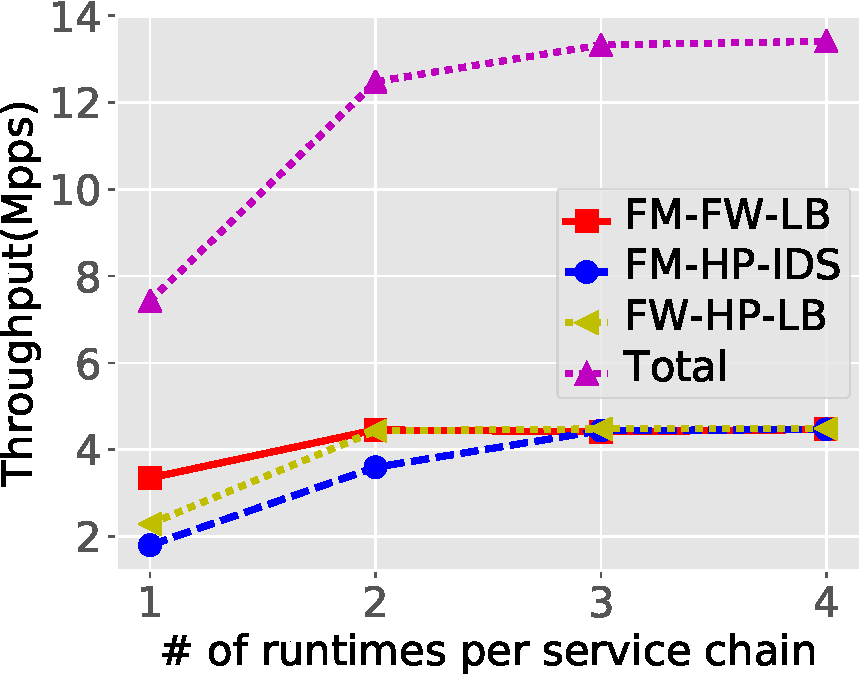
\includegraphics[width=\columnwidth]{figure/revised-throughput-test.pdf}
%	\caption{Packet processing throughput.}
  %(\textbf{FM}: Flow Monitor. \textbf{HP}: HTTP Parser. \textbf{FW}: Firewall. \textbf{LB}: Load Balancer. \textbf{IDS}: Intrusion Detection System.)
%\label{fig:normal-case-eval}
%\end{figure}

\begin{figure}[!t]
 \begin{subfigure}[t]{0.475\linewidth}
   \centering
   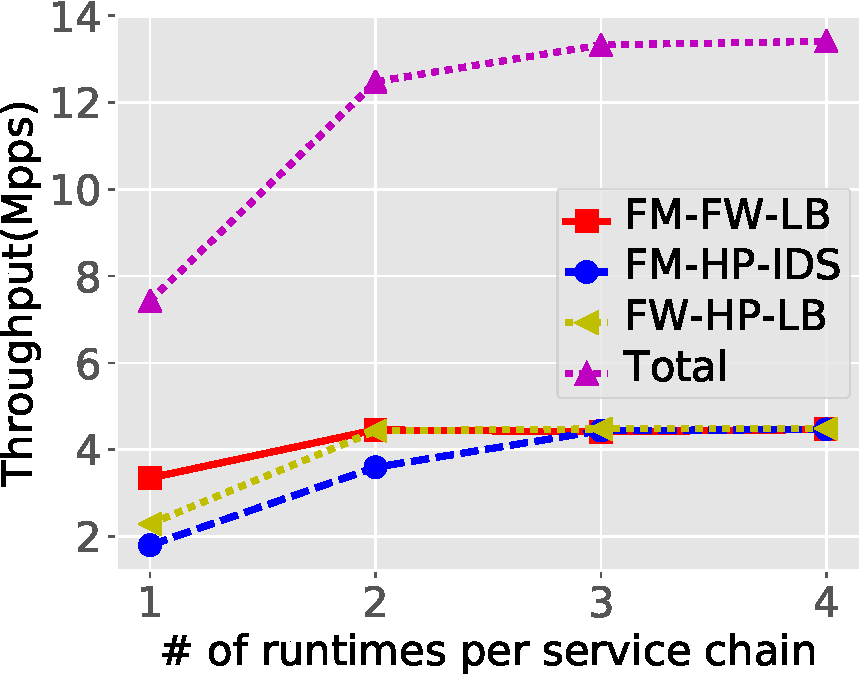
\includegraphics[width=\columnwidth]{figure/revised-throughput-test.pdf}
   \caption{}\label{fig:normal-case-eval} \end{subfigure}\hfill
  \begin{subfigure}[t]{0.505\linewidth}
   \centering
   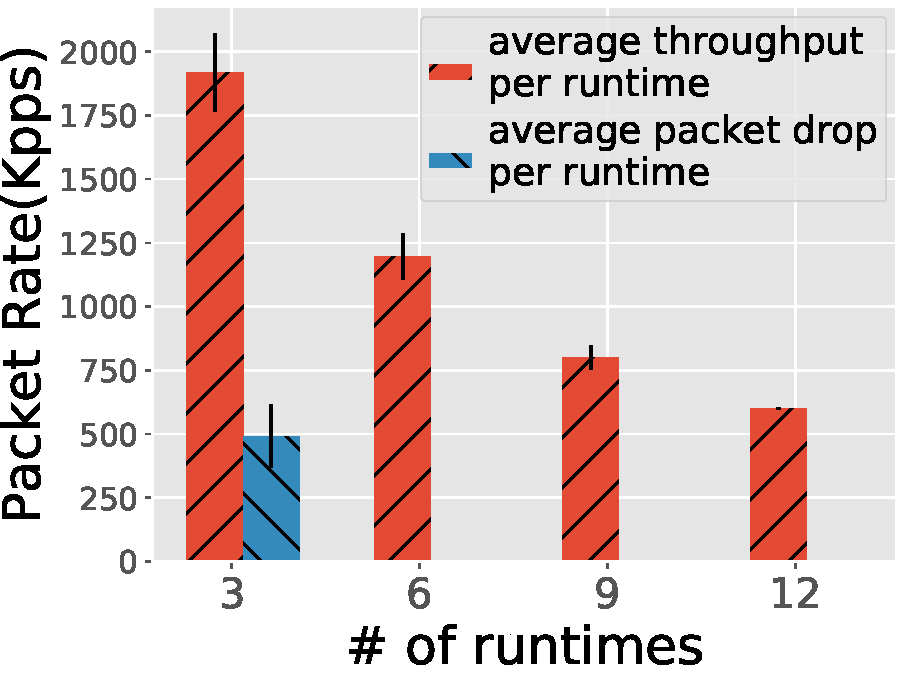
\includegraphics[width=\columnwidth]{figure/Mixtest.pdf}
   \caption{}\label{fig:mix-work-flow}
  \end{subfigure}
\caption{ Packet processing throughput.} %(a) The total time to migrate different numbers of flows concurrently on three runtimes. (b) The flow migration performance of NFActor. Each flow in NFActor runtime goes through the same service chain as in Figure \ref{fig:tot-mig}. OpenNF controlls PRADS asset monitors. The flow packet rate is 20pps.}
\label{fig:mig-perf}
\end{figure}



 %\begin{figure}[!t]
%	\begin{subfigure}[t]{0.49\linewidth}
%		\centering
%		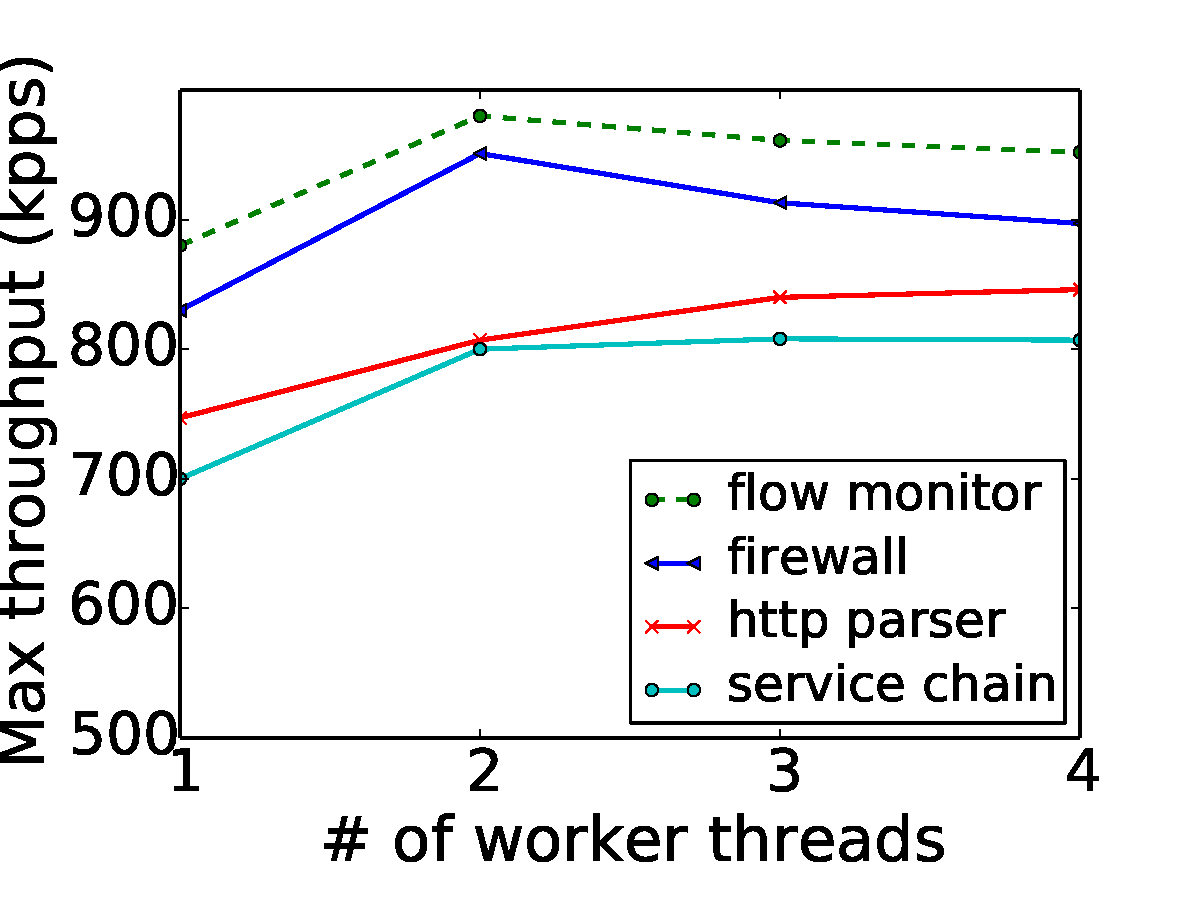
\includegraphics[width=\columnwidth]{figure/nf_throughput_evaluation.pdf}
%		\caption{Packet processing capacity of a single \nfactor~runtime system running with different number of worker threads.}\label{fig:normal-performance} \end{subfigure}\hfill
%	 \begin{subfigure}[t]{0.49\linewidth}
%		\centering
%		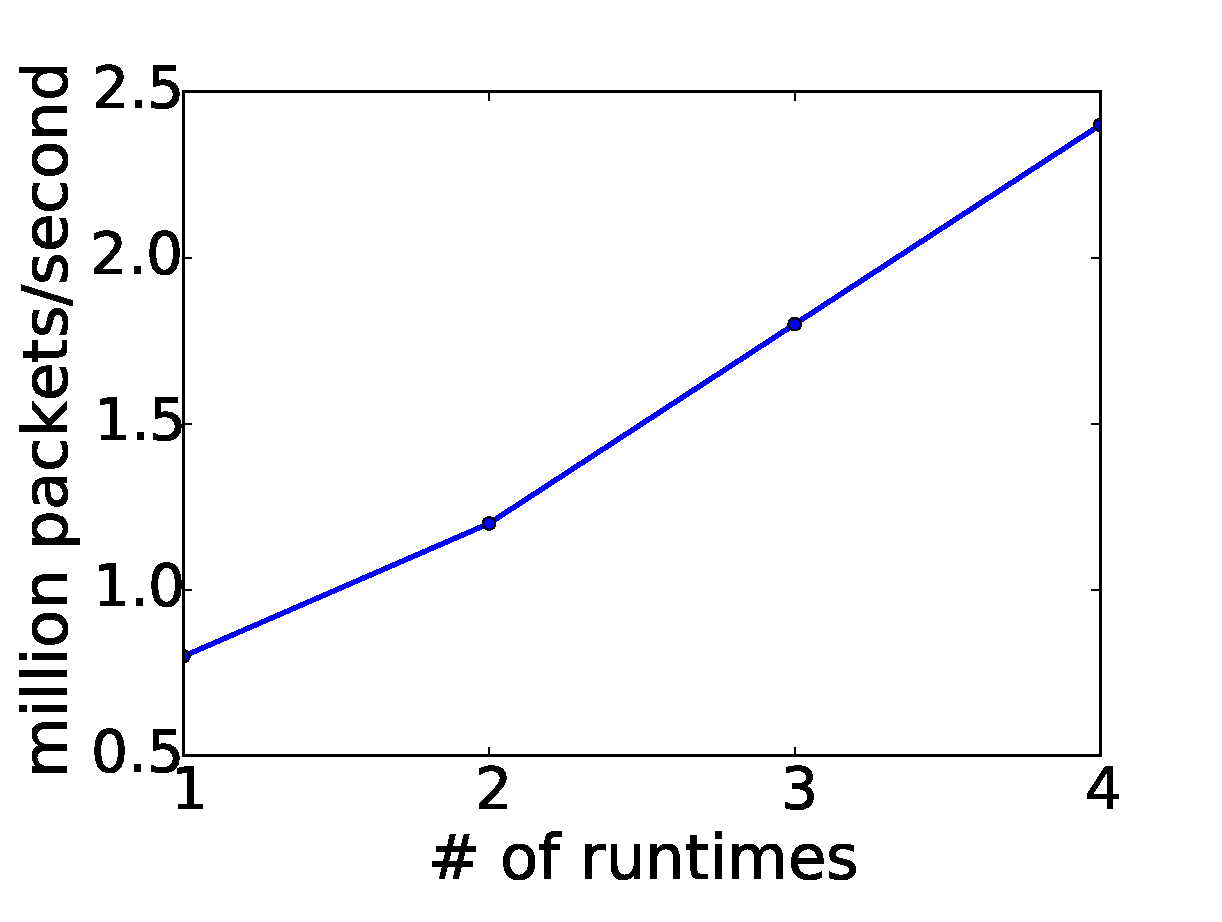
\includegraphics[width=\columnwidth]{figure/runtime_pktthroughput.pdf}
%		\caption{Aggregate packet processing capacity of several \nfactor~runtimes.}\label{fig:scalability-performance}
%	 \end{subfigure}
%\caption{The performance and scalability of \nfactor~runtime, without enabling flow migration }
%\label{fig:performance}
%\end{figure}

We run six virtual switches on one server for dispatching flows to runtimes, run runtimes on other servers, and implement a traffic generator to produce flows to be sent to virtual switches. The flows consist of 64 byte data packets. We deploy three service chains, `flow monitor (FM) $\rightarrow$ firewall (FW) $\rightarrow$ load balancer (LB)', `flow monitor (FM) $\rightarrow$ HTTP parser (HP) $\rightarrow$ IDS', and `flow monitor (FM) $\rightarrow$ HTTP parser (HP) $\rightarrow$ load balancer (LB)'.\footnote{\nfactor~can handle service chains with branches similarly, due to encapsulating each service chain entirely in one flow actor and the run-to-completion scheduling strategy in runtimes. We evaluate simple service chains without branches which represent the mainstream \cite{hwang2015netvm, martins2014clickos}.} The same number of flows are processed by each of the service chains. We do not enable flow replication in this set of experiments. % and use the same number of runtimes to process packets for each service chain.


We first evaluate the packet processing throughput of \nfactor~using uniform flows, each produced at 10pps (packets per second), lasting for 10 seconds. We inject an overall rate of all flows around $14Mpps$ (60K flows) into virtual switches, %\chuan{14*64*8=7168, why is this close to line rate of 20Gbps for the two NICs of a server? Answer: because on the ethernet, the size of the packet is increased to larger than 80bytes.}
 which approaches line-rate of the server NICs. We evaluate the throughput when different numbers of runtimes are deployed for each service chain. %Since each runtime can handle at most 50000 flows, we scale up the number of runtimes with the increase of flows.

%For each service chain, we run two traffic generators to generate traffic into the service chain, resulting in a maximum throughput at around 4.4Mpps.


Fig.~\ref{fig:normal-case-eval} shows that %all flows using each service chain can be timely processed.
 when there are more than 2 to 3 runtimes for each service chain, the total packet processing capacity of the runtimes is larger than the incoming flow rate (about $14Mpps$), leading to a stabilizing overall throughput about $14Mpps$.  %starting with 2 or 3 runtimes implies that the amount of the input traffic injected into the service chains is smaller than the total packet processing capacity of these service chains when each of these two chains are scaled with more than 2 runtimes. %The total throughput of \nfactor when handling three service chains easily scale up to around 14Mpps, which basically saturate a 10Gb NIC card, therefore achieving line-rate throughput. Therefore~\nfactor can scale well and satisfies the line-rate processing requirement of modern NFV system.
 In addition, we start to observe zero packet loss for all the three service chains when the number of runtimes is scaled up to 3.



 We next evaluate packet processing throughput with flows whose duration spans 10 seconds to one minute, %, with a 10 second step. The
 %flow arrival rate varies from 1000 flows to 5000 flows \chuan{why do you need to vary the flow arrival rates? I think this experiment should be done using static total flow numbers; you can comment this clause out andrevise the total number of flows injected to the concurrent number},
flow rate varies from 1kpps to 2kpps, %with a 1000-flow step.
 and packet size varies among 64 bytes, 128 bytes and 256 bytes. The total number of injected flows is 550K.
 The runtimes are configured with a service chain `flow monitor $\rightarrow$ HTTP parser $\rightarrow$ IDS'. Fig.~\ref{fig:mix-work-flow} shows the average throughput and packet drop of each runtime, when different numbers of runtimes are deployed for each service chain. An error bar indicates the standard deviation. We can see that the flow processing load is quite balanced among different runtimes (using our simple round-robin scheduling algorithm) and the runtimes can handle all the incoming flows when the number of runtimes is scaled up to six (zero loss). The primary reason that the round-robin scheduling works well enough even in case of non-uniform flows is that the total number of injected flows is large enough (550K), a common case in high-speed NFV systems, where large and small flows balance out.

These results exhibit high efficiency of the runtime design and flow migration protocol in \nfactor. % enabling close to line-rate flow processing. % good packet processing performance achieved by~\nfactor is primarily due to our efficient actor design.
 The development of \nfactor~has gone through a few trials and errors. In our previous version of \nfactor~design and prototype implementation using Libcaf \cite{caf}, we used 4 worker threads per runtime. Compared with the old design, our current design with one worker thread per runtime can achieve up to 4x throughput. We believe the reason is that the customized actor library and the single worker thread design completely eliminate the overhead of multi-threaded contention for shared resource, \ie actor's mailbox. % enabling current version to out-perform the previous version.

% We believe the reason is that the combination of our customized actor library and the DPDK-based reliable message passing eliminates a lot of overhead associated with actor processing. \chuan{the reason you gave is not relevant to 4 worker threads per runtime}
%The traffic generator generates  generate the same amount of traffic to each service chain.  using differnt number of runtimes, running three service chains. The traffic generators generates flows each lasts for 10 second with a 20 pps (packet per second) flow rate. The packet size is 64 byte. We increase the number of concurrently generated flows to generate packets at around 14Mpps, reaching NIC line-rate. We set up different number of runtimes and configure runtimes with different service chains and calculate the cumulative packet rate from all the runtimes. From \ref{fig:normal-case-eval}, we can see that the runtime in~\nfactor can scale almost linearly and achieve almost line-rate processing when scaled up to 9 runtimes. Therefore,~\nfactor has good packet processing throughput and can satisfy the stringent requirement of modern NFV system.

% reach   with a uniform We can see that the packet processing throughput scales almost linearly as the number of runtime increases, until normal case performance of running \nfactor~framework. Each flow in the generated traffic has a 10 pps (packet per second) per-flow packet rate. We vary the number of concurrently generated flows to produce varying input traffics. In this evaluation, we gradually increase the input packet rate to the \nfactor~cluster and find out the maximum packet rate that the \nfactor~cluster can support without dropping packets. In figure \ref{fig:normal-performance}, the performance of different NF modules and the service chain composed of the 3 NF modules are shown. Only one \nfactor~runtime is launched in the cluster. It is configured with different number of worker threads. In figure \ref{fig:scalability-performance}, we create different number of \nfactor~runtimes and configure each runtime with 2 worker threads. Then we test the performance using the entire service chain.

%From figure \ref{fig:normal-performance}, we can learn that the packet throughput decreases when the length of the service chain is increased. Another important factor to notice is that the \nfactor~runtime does not scale linearly as  the number of worker threads increases. The primary reason is that inside a \nfactor~runtime, there is only one packet polling thread. As the number of input packets increases, the packet polling thread will eventually become the bottleneck of the system. However, \nfactor~runtime scales almost linearly as the total number of \nfactor~runtimes increases in the cluster. When the number of runtimes is increased to 4 in the system, the maximum packet throughput is increased to 2.4M pps, which confirms to the line speed requirement of NFV system.

\subsection{Time Consumption for Flow Migration}
\label{sec:fmp}

 \begin{figure}[!t]
	\begin{subfigure}[t]{0.49\linewidth}
		\centering
		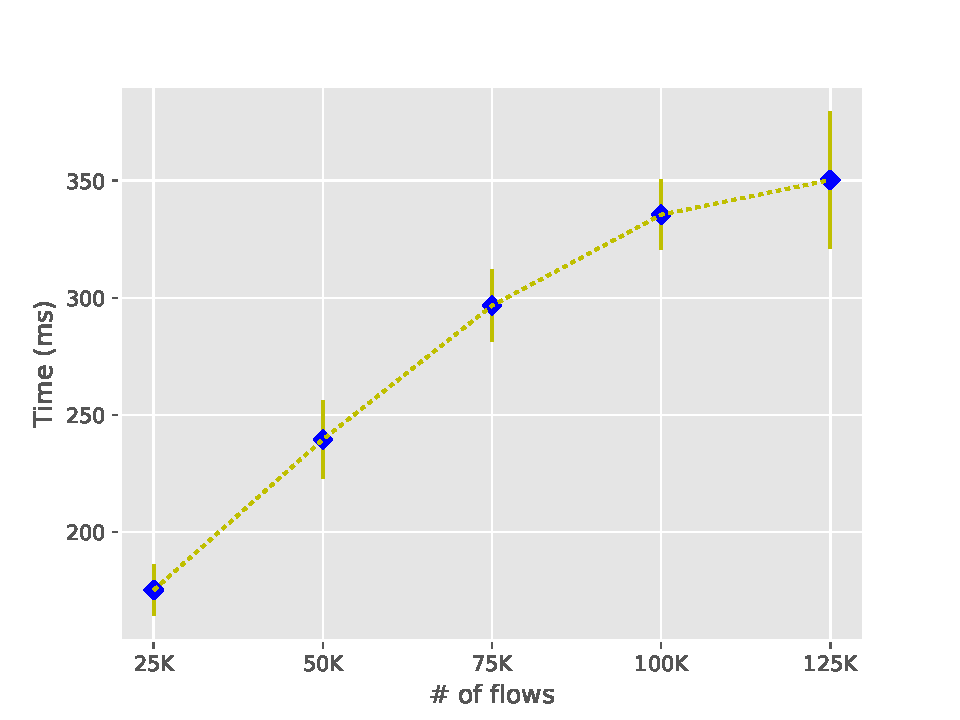
\includegraphics[width=1.05\columnwidth]{figure/Migration.pdf}
		\caption{}\label{fig:tot-mig} \end{subfigure}\hfill
	 \begin{subfigure}[t]{0.49\linewidth}
		\centering
		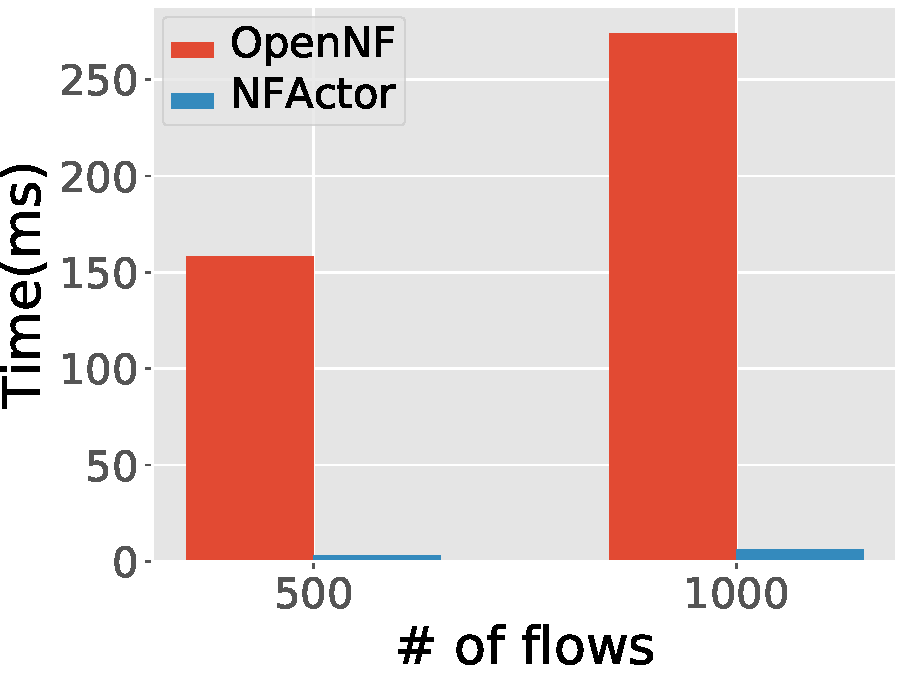
\includegraphics[width=\columnwidth]{figure/Compare.pdf}
		\caption{}\label{fig:compare-opennf}
	 \end{subfigure}
\caption{ Time consumption for flow migration.} %(a) The total time to migrate different numbers of flows concurrently on three runtimes. (b) The flow migration performance of NFActor. Each flow in NFActor runtime goes through the same service chain as in Figure \ref{fig:tot-mig}. OpenNF controlls PRADS asset monitors. The flow packet rate is 20pps.}
\label{fig:mig-perf}
\end{figure}


To inspect performance of flow migration in \nfactor, we show time taken for migrating large numbers of flows. We run three runtimes on each server, configured to run service chain ``firewall $\rightarrow$ http parser $\rightarrow$ load balancer''. The traffic generator produces flows of rate $20pps$ each, and virtual switches dispatch flows evenly to runtimes on one of the servers. %, therefore each runtime on the first server processes approximately the same number of flows.
 After the traffic stabilizes, the coordinator asks all runtimes on that server to migrate all their flows to three runtimes on another server, concurrently.

We vary the number of flows injected to each runtime and show in Fig.~\ref{fig:tot-mig} completion time for migrating all flows from a runtime, averaged over all three runtimes. We can see that it takes $350$ms for migrating about $125000$ flows (with 2.5Mpps packet processing throughput). %\chuan{complete xx. how do you come up with `even when migrating more than 300000 flows, with 6Mpps processing throughput'?}.
The time only increases sublinearly with the increase of flows. Considering the migration is concurrently carried out among three pairs of runtimes, the results show good efficiency of our distributed flow migration and the following design:
%The key reason that~\nfactor is able to achieve such a good flow migration performance is because
(i) flow states are directly copied into remote actor messages without the need for serialization and deserialization, and (ii) remote actor messages are directly encapsulated in L2 network packets and transmitted using DPDK. %with high-performance packet I/O.

We also observe zero packet loss throughout the experiment. %keep the number of lost packet due to migration target buffer overflow or packet reordering. Throughout the entire experiment, this number is zero.
 This shows that the collective buffer of a capacity of 4096 packets (for all migration target actors to buffer received flow packets in a runtime before the request in the 3rd request-response step is received), is sufficient even when migrating a large number of flows. %This buffer size is large enough to \chuan{justify why maintaining this buffer size per actor is reasonable}.

We also compare \nfactor~with OpenNF \cite{gember2015opennf} for flow migration. We send the same number of flows to \nfactor~runtimes and NFs controlled by OpenNF, and present the total time to migrate these flows in Fig.~\ref{fig:compare-opennf}.\footnote{We were not able to test under large numbers of flows due to unexpected failures when running OpenNF, possibly due to our lack of experience in operating its authors' program.} Flow migration in \nfactor~takes much less time. Though this may not be a very fair comparison as OpenNF uses legacy NFs while \nfactor~relies on NFs implemented following our design, we believe the results are still illustrative.

%Each flow in NFActor runtime goes through the same service chain as in Figure \ref{fig:tot-mig}. OpenNF controlls PRADS asset monitors. The flow packet rate is 20pps.

%the migration completion time of \nfactor~is more than 50\% faster than OpenNF.  This performance gain primarily comes from the simplified migration protocol design with the help of actor framework. In \nfactor, a flow migration process only involves transmitting 3 request-responses. Under light workload, the flow migration can complete within several hundreds of microseconds. Under high workload, \nfactor~runtime system controls the maximum number of concurrent migrations to control the migration workload, which may increase the migration performance as indicated in figure \ref{fig:avg-time-batch-mig}. All of these factors contribute to the improved flow migration performance of \nfactor~framework.

%three runtimes and migrate flows from one runtime on the firs

%We present the evaluation result of flow migration in this section. In order to evaluate flow migration performance, we initialize the cluster with 2 runtimes running with 2 worker threads and then generate flows to one of the runtimes. Each flow is processed by the service chain consisting of all the 3 NF modules. We generate different number of flows, each flow has the same per-flow packet rate. In order to see how the evaluation performs under different per-flow packet rate, we also tune the per-flow packet rate with 10pps, 50pps and 100pps. When all the flows arrive on the migration source runtime. The migration source runtime starts migrating all the flows to the other runtime in the cluster. We calculate the total migration time and the average per-flow migration time. In order to control the workload during the migration, the runtime only allows 1000 concurrent migrations all the time. The result of this evaluation is shown in figure \ref{fig:mig-perf}.

%We can see that as the number of migrated flows increase, the migration completion time increases almost linearly. This is because the average flow migration time remains almost a constant value and the runtime controls the maximum number of concurrent migrations. Note that when the system is not overloaded at all (100 flows), the average flow migration completion time is as small as 636us.

%When the per-flow packet rate is 100pps, the maximum number of flows that we use to evaluate the system is 6000. Continuing the evaluation with 8000 and 10000 flows just overloads the runtime as shown in figure \ref{fig:normal-performance}.

 %\begin{figure}[!t]
 %\begin{subfigure}[t]{0.49\linewidth}
%		\centering
%		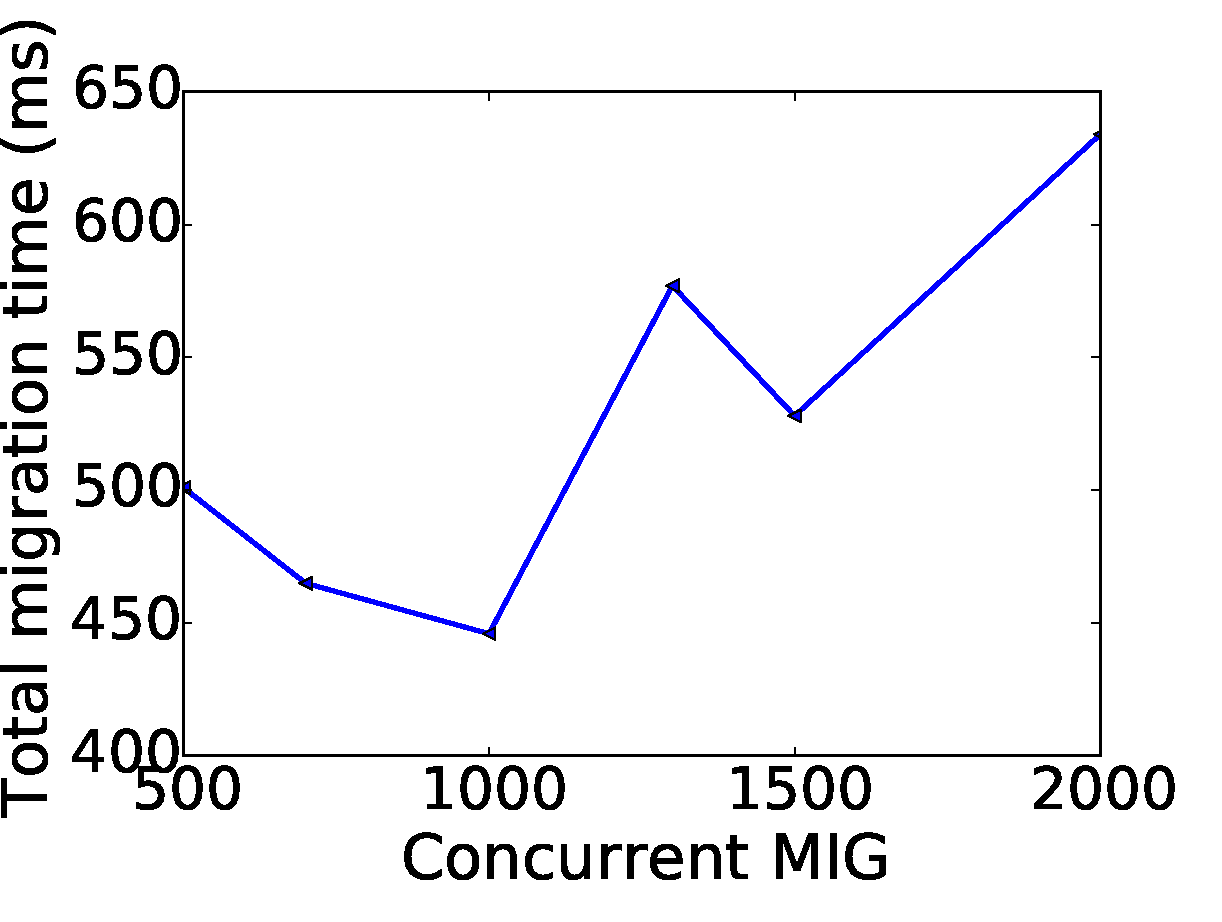
\includegraphics[width=\columnwidth]{figure/vary_batch_tot_migration_time.pdf}
%		\caption{The total time to migrate all the flows when changing the maximum concurrent migrations.}\label{fig:avg-time-batch-mig}
%	 \end{subfigure}\hfill
%	 \begin{subfigure}[t]{0.49\linewidth}
%	\centering
%		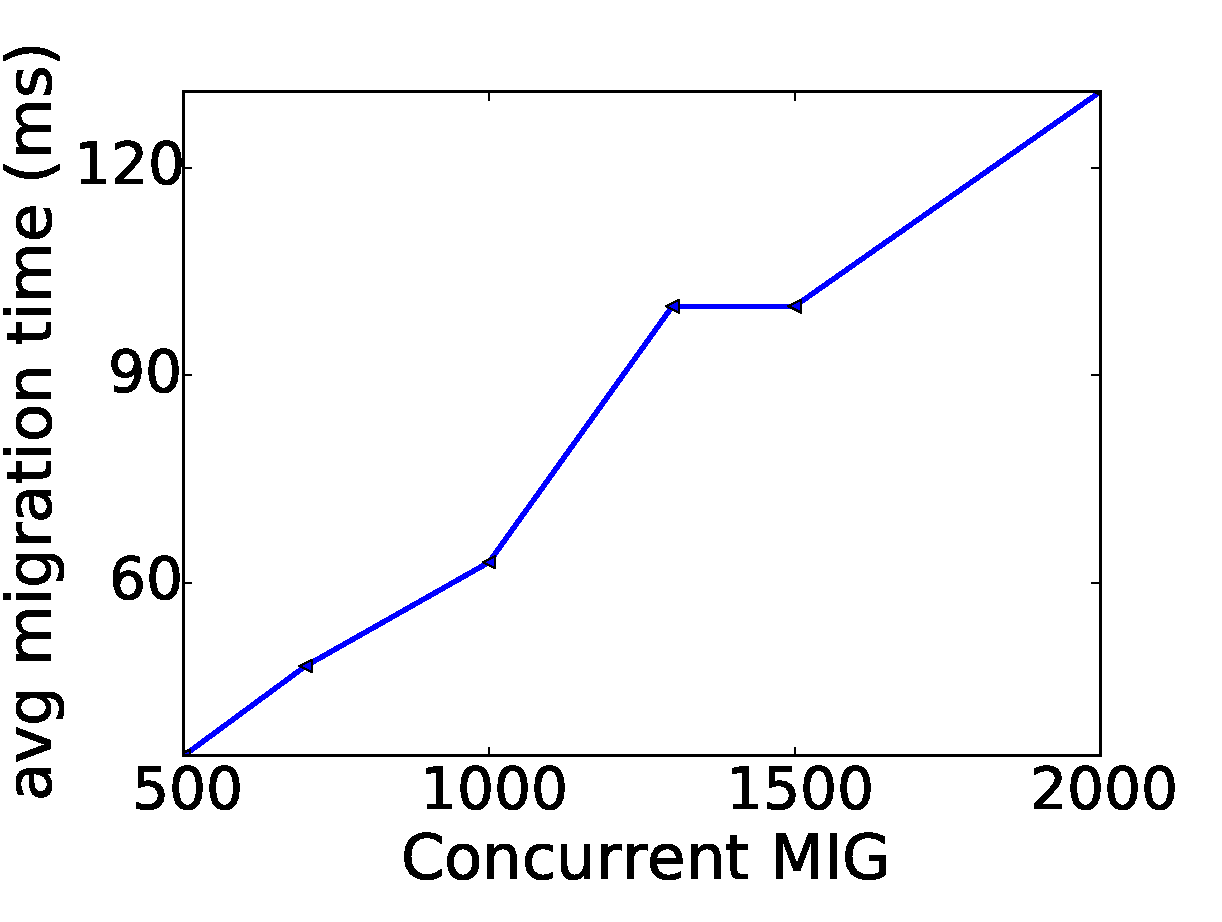
\includegraphics[width=\columnwidth]{figure/vary_batch_avg_migration_time.pdf}
%		\caption{The average flow migration time of a single flow when changing the maximum concurrent migrations.}\label{fig:avg-mig-batch} \end{subfigure}
%	\caption{The flow migration performance of \nfactor~when changing the maximum concurrent migrations.}
%\label{fig:mig-perf}
%\end{figure}

%Since we control the number of concurrent migrations, we also want to see what happens if we change the number of concurrent migrations. We generate 6000 flows, each with 50 pps per-flow packet rate, and change the the number of concurrent migrations. The result of this evaluation is shown in fig \ref{fig:mig-perf}. As we can see from fig \ref{fig:avg-mig-batch}, increasing the maximum concurrent migrations increase the average flow migration completion time. However, whether the total flow migration completion time increased depends on the total number of flows that wait to be migrated. From the result of fig \ref{fig:avg-time-mig}, the choice of 1000 concurrent migrations sits in the sweat spot and accelerates the overall migration process.

 %\begin{figure}[!t]
%		\centering
%		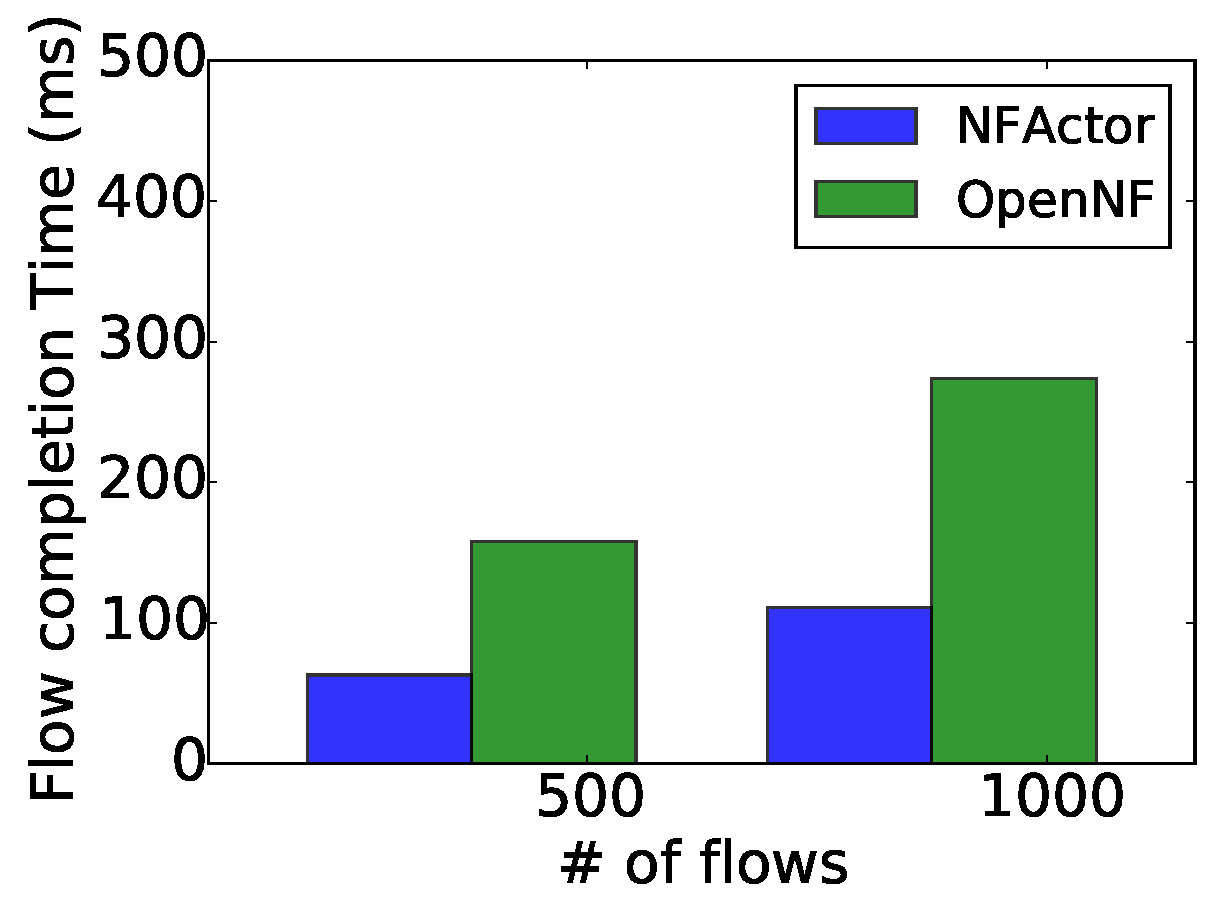
\includegraphics[width=0.6\columnwidth]{figure/opennf_nfactor_cmpFlowtime.p%df}
%		\caption{The flow migration performance of \nfactor. Each flow in \nfactor~runtime goes through the service chain consisting of the 3 customzied NF modules. OpenNF controlls PRADS asset monitors.}
%\label{fig:compare-opennf}
%\end{figure}

%Finally, we compare the flow migration performance of \nfactor~against OpenNF \cite{gember2015opennf}. We generate the same number of flows to both \nfactor~runtimes and NFs controlled by OpenNF and calculate the total time to migrate these flows. The evaluation result is shown in figure \ref{fig:compare-opennf}. Under both settings, the migration completion time of \nfactor~is more than 50\% faster than OpenNF.  This performance gain primarily comes from the simplified migration protocol design with the help of actor framework. In \nfactor, a flow migration process only involves transmitting 3 request-responses. Under light workload, the flow migration can complete within several hundreds of microseconds. Under high workload, \nfactor~runtime system controls the maximum number of concurrent migrations to control the migration workload, which may increase the migration performance as indicated in figure \ref{fig:avg-time-batch-mig}. All of these factors contribute to the improved flow migration performance of \nfactor~framework.

\subsection{Throughput during Dynamic Scaling}

%\begin{figure}[!t]
%	\centering
%	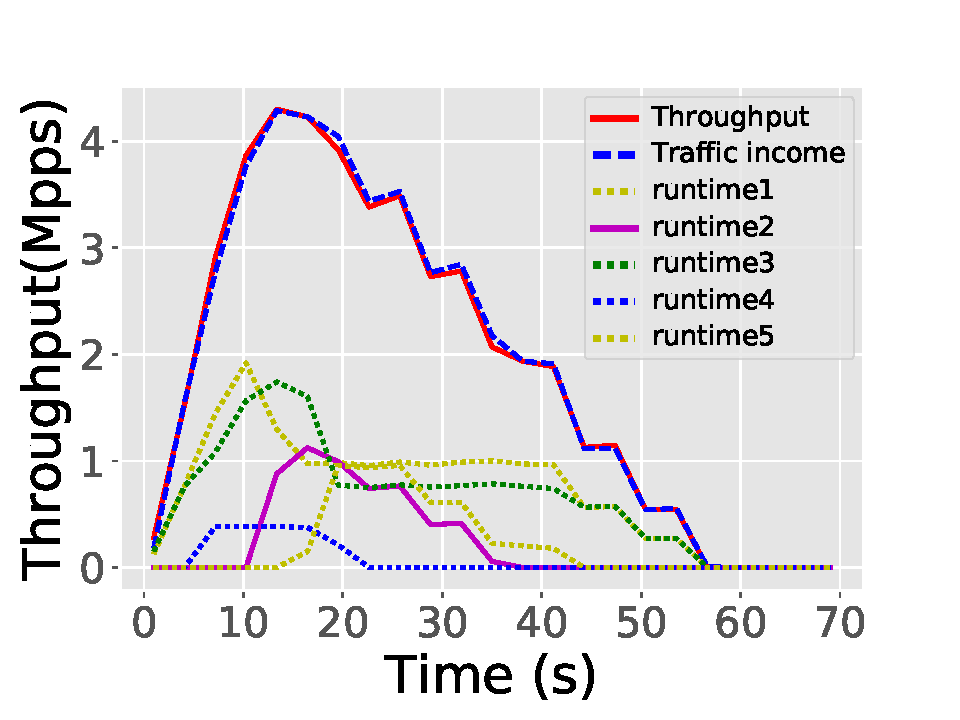
\includegraphics[width=\columnwidth]{figure/Scale.pdf}
%	\caption{Throughput during dynamic scaling.}
%\label{fig:normal-case-scale}
%\end{figure}

\begin{figure*}[!t]
\captionsetup{width=0.3\textwidth}
\begin{center}
\begin{minipage}[t]{0.355\linewidth}
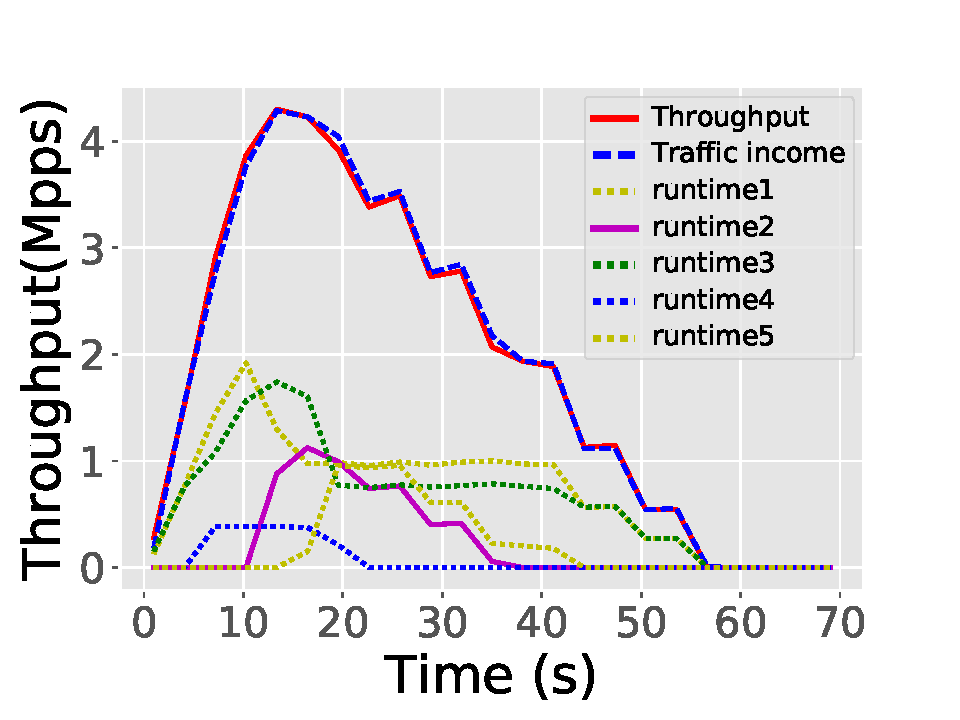
\includegraphics[width=1\textwidth]{figure/Scale.pdf}
	\caption{Throughput during dynamic scaling.}
\label{fig:normal-case-scale}
\end{minipage}
\hfill
\begin{minipage}[t]{0.615\linewidth}
 \begin{subfigure}[t]{0.48\linewidth}
		\centering
		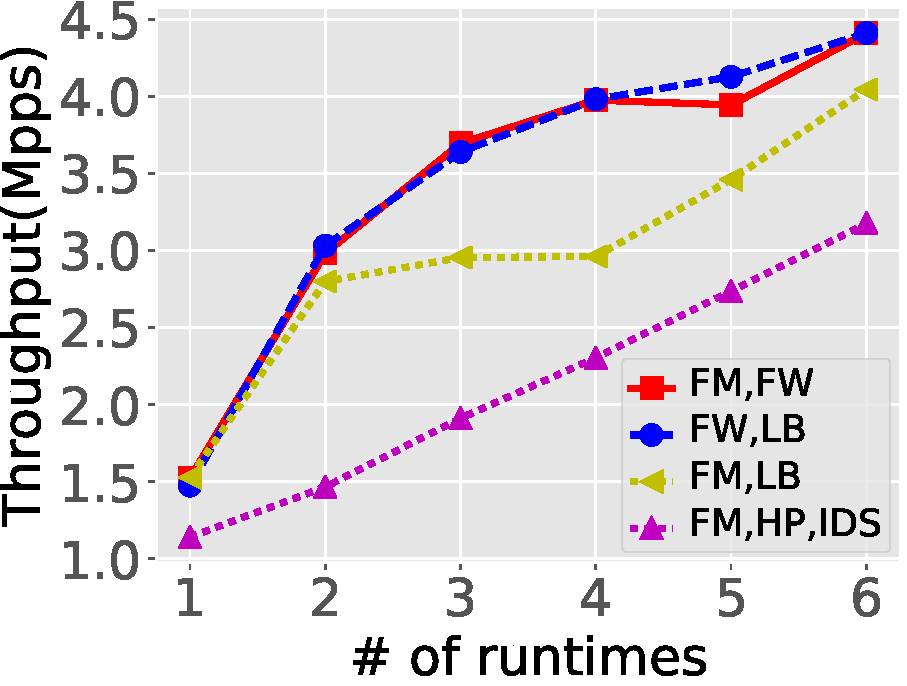
\includegraphics[width=\columnwidth]{figure/ReplicaTP.pdf}
		%\caption{The packet throughput of a \nfactor~cluster when replication is enabled. }
		\caption{}\label{fig:rep-scale}
	 \end{subfigure}\hfill
	 \begin{subfigure}[t]{0.49\linewidth}
	\centering
		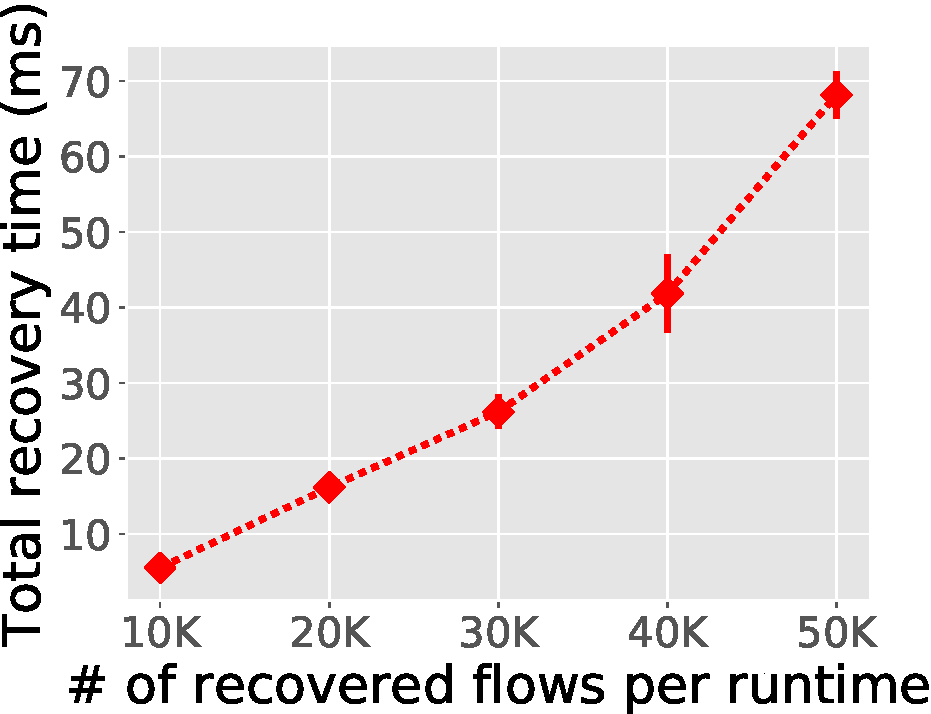
\includegraphics[width=1\columnwidth]{figure/Recover.pdf}
		%\caption{The recovery time of three failed runtimes under different settings. The tuple on the $x$ axis represents the number of the runtime used in the evaluation and the total input packet rate. }
		\caption{}\label{fig:rep-recovery} \end{subfigure}
	\caption{Performance of flow migration}
\label{fig:rep-perf}
\end{minipage}
\end{center}
\vspace{-5mm}
\end{figure*}


We further evaluate performance of dynamic scaling mechanism in \nfactor. The traffic generator produces a varying number of flows overtime. Each flow has a rate of 20pps, lasting 60 seconds. The runtimes are configured with service chain ``firewall $\rightarrow$ HTTP parser $\rightarrow$ IDS''. Fig.~\ref{fig:normal-case-eval} shows that the cluster is scaled up to 6 runtimes to handle the peak rate. We observe that whenever a runtime is overloaded (runtime 1 and runtime 4), our mechanism promptly resolves the hotspot (considering each flow lasts 60s). %, without the efficient and distributed flow migration. ~\nfactor would not be able to achieve this, but continue to be overloaded for a long period of time, resulting in severe performance drop.

We further observe in our experiment that the CPU usage of the coordinator remains under 5\%, due to its lightweight design.


\subsection{Performance of Flow Replication}
\label{sec:rp}

\begin{comment}
 \begin{figure}[!t]
 \begin{subfigure}[t]{0.49\linewidth}
		\centering
		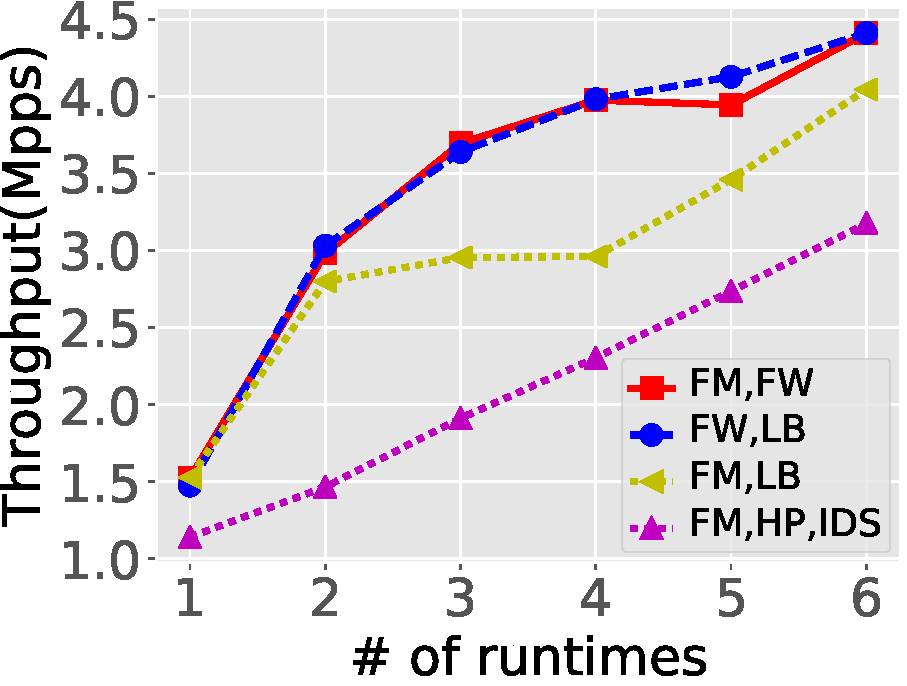
\includegraphics[width=\columnwidth]{figure/ReplicaTP.pdf}
		%\caption{The packet throughput of a \nfactor~cluster when replication is enabled. }
		\caption{}\label{fig:rep-scale}
	 \end{subfigure}\hfill
	 \begin{subfigure}[t]{0.49\linewidth}
	\centering
		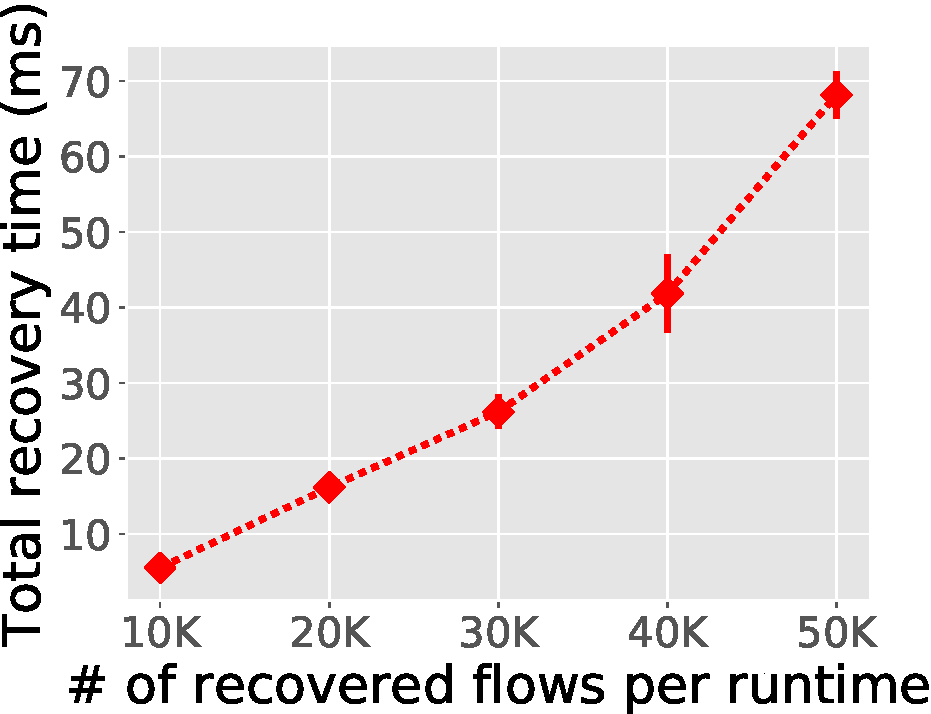
\includegraphics[width=\columnwidth]{figure/Recover.pdf}
		%\caption{The recovery time of three failed runtimes under different settings. The tuple on the $x$ axis represents the number of the runtime used in the evaluation and the total input packet rate. }
		\caption{}\label{fig:rep-recovery} \end{subfigure}
	\caption{Performance of flow migration}
\label{fig:rep-perf}
\end{figure}
\end{comment}
%\chuan{Fig.~\ref{fig:rep-scale}: better to make the service chains in Fig. \ref{fig:normal-case-eval} and this figure the same, such that readers can compare the difference with and without flow replication}


%both in terms of overall packet processing throughput achieved during flow replication and the recovery time when a runtime fails.  Therefore we set up several runtimes on a server, configure each of these runtimes with a dedicated replica runtime on anther server.

We next enable flow replication in \nfactor. The traffic generator produces 300K flows with a flow rate of 30pps.  % to generate traffic to the runtimes being replicated, and
Four different service chains are used in this experiment.
Three runtimes are running on each server.
%calculate the accumulated packet throughput from the replica.

Fig.~\ref{fig:rep-scale} shows that with the increase of runtimes deployed for each service chain, the packet processing throughput from runtimes running each service chain increases, but is always lower than the throughput if no flow replication is in place. %. For runtimes running service chains consisting of lightweight NFs (\eg, flow monitor, firewall and load-balancer), the overall throughput gradually increases to around 4Mpps
% 9Mpps. %\chuan{give the largest throughput if not doing flow replication}.
At the peak throughput, the bandwidth on the L2 network has been saturated and becomes the bottleneck. This is because for each input packet, an additional packet is transmitted from the original runtime to the replication target runtime, %at least two output packets,
 containing the flow states and the output packet processed by the flow actor. These packets consume additional bandwidth in the system. %Being transmitted through reliably to the remote side, these packets are also appended with a header (the average size is 25bytes for each packet), further increase the bandwidth usage.
 We believe such additional bandwidth consumption is unavoidable if to ensure the % that our flow replication scheme remains its applicability because it achieves the
 output-commit property. To mitigate this issue, a flow actor can replicate its flow states after it has processed multiple packets, at the cost of weaker flow state consistency. %is weaker,~\nfactor could be easily adapted to use a light-weight replication scheme, that replicates the the flow state after it has processed multiple packets, to increase the throughput.

The biggest advantage brought by \nfactor's flow replication is the fast recovery time in case of failures. %Following the settings as in Figure~\ref{fig:rep-scale},
We emulate a server crash by shutting down the server, and recover flows processed by failed runtimes on their replicas on other servers. Fig.~\ref{fig:rep-perf} shows that 50000 flows can be recovered within tens of milliseconds. This is because flow recovery in \nfactor~is extremely lightweight, involving only one request-response pass between the replica runtime and the virtual switch. % for each replicated flow actor.

We do not show results evaluating failure resilience of the coordinator and the virtual switches, since their handling in cases of failures is mostly standard as in the literature.

%To evaluate~\nfactor's flow replication, we configure the virtual switch to generate output packets to runtimes on the first server. For each runtime on the first server, we configure a replica runtime on the second server, and let each runtime replicate its flows to the corresponding replica runtime. We calculate the cumulative packet processing throughput during flow replication. The result is shown in Figure~\ref{fig:rep-scale}. We can see that the scalability during flow replication is not as good as the result achieved when replication is disabled. The replication throughput can achieve an almost linear scalability when there are smaller than four runtimes running in a single server, but the scalability starts to degrade when more runtimes are used. The primary reason is because the bandwidth consumption on the L2 network is way higher than normal case evaluation. To ensure output-commit property, for each input packet, the runtime generates at least two output packets, containing the flow state and the output packet processed by the flow actors.

%~\nfactor replicates the flow state for each processed packet using a reliable message passing module. The number of transmitted packets by the reliable message passing module is actually two times the number of the input packets. To reliably transmit flow state and the processed packet, the runtime also needs to add a header for each remote actor message, which is 52 byte long in our implementation. All these reasons contribute to a much larger bandwidth that are actually delivered over the network, which may result in potential packet drops.

%In this section, we present the flow replication evaluation result. In our evaluation, the actor creates a flow snapshot for every 10 flow packets that it has processed. Then it sends the flow state snapshot to the replica storage. In this evaluation, we first generate flows to the \nfactor~cluster to test the maximum throughput of a \nfactor~cluster when enabling replication. Then we calculate the recovery time of failed \nfactor~runtime. The recovery time is the from time that the controller detects a \nfactor~runtime failure, to the time that the recovered \nfactor~finishes replaying all of its replicas and responds to the controller to rejoin the cluster. Through out this evaluation, the runtime uses the service chain consisting of the 3 NF modules to process the flow. The result of the evaluation is shown in figure \ref{fig:rep-perf}.

%In figure \ref{fig:rep-scale}, we can see that there is an obvious overhead to enable replication on \nfactor~runtimes. The overall throughput when replication is enabled drops around 60\%. This is due to the large amount of replication messages that are exchanged during the replication process. Internally, the replication messages are sent over Linux kernel networking stack, which involves data copy and context switching, thus increasing the performance overhead of using replication. However, the overall throughput when replication is enabled could scale to 850K pps when 4 runtimes are used, which is enough to use in some restricted settings.

%Finally, figure \ref{fig:rep-recovery} shows the recovery time of \nfactor~runtime when replication is enabled. We found that the recovery time remains a consistent value of 3.3s, no matter how many runtimes are used or how large the input traffic is. The reason of this consistent recovery time is that the \nfactor~runtime maintains one replica on every other \nfactor~runtimes in the cluster. During recovery, several recovery threads are launched to fetch only one replica from another runtime. Then each recovery thread independently recovers actors by replaying its own replica. In this way, the recovery process is fully distributed and scales well as the number of replica increases. Note is that the average time it takes for a recovered runtime to fetch all the replicas and recover all of its actors is only 1.2s. So actually around 2.1s is spent in container creation and connection establishment.


\subsection{Other Applications}
\label{sec:applications}



In addition, we build two applications based on \nfactor, which exploit its lightweight, distributed flow migration capability to achieve useful functionalities. %, including live NF update, reduce output bandwidth for deduplication NF and ensure reliable and safe MPTCP processing. We evaluate and demonstrate these new applications in our evaluation.

\vspace{1mm}
\noindent\textbf{Live NF update.} %NF often needs to be updated (\eg, software version, important NF configuration files), existing systems would typically migrate flows away, stop the NF and then relaunching it.
 \nfactor~can achieve dynamic NF update (\eg, software version, important NF configuration files) without interfering active flows, by dynamically migrating the flows out to a replica runtime, performing update and migrating the flows back. Fig.~\ref{fig:dynamic-update} illustrates the throughput of a runtime running a firewall NF, during dynamic update of its firewall rule. No active flows are dropped during the update with \nfactor, while significant throughput drop occurs if shutting down the firewall for its update.

\vspace{1mm}
\noindent\textbf{MPTCP sub-flow processing.} When an MPTCP \cite{wischik2011design} flow traverses an NFV system, its sub-flows may be sent to different NF instances for processing. Some network functions require all subflows to be processed by the same instance, \eg, IDS. % requires that all subflows of the same MPTCP flow to be examined by the same IDS instance to detect potential netowrk attacks.
In \nfactor, we can add an MPTCP sub-flow detection function to each flow actor, such that when the flow actor processes the first packet of a flow, it can check whether it belongs to an MPTCP flow. If so, the flow actor performs a consistent hashing using the MPTCP header to decide a migration target runtime in the cluster, and migrates the flow to the target. In this way, different sub-flows belonging to the same MPTCP flow can be processed by the same flow actor. This is hard to be achieved in the existing NFV systems without significant central coordination. %, since flows can not initiate active migration request by themselves.

In the experiment of Fig.~\ref{fig:mptcp}, we inject a total number of about 320K MPTCP flows to 3 runtimes. With subflow detection enabled, the total number of correctly processed MPTCP flows is always the same as the number of input flows, \ie, those whose subflows are all processed by the same runtime. Without this detection, most of the subflows are processed by different runtimes. % therefore only a small amount of MPTCP flows are correctly processed.

\begin{figure}[!t]
\begin{subfigure}[t]{\linewidth}
   \centering
   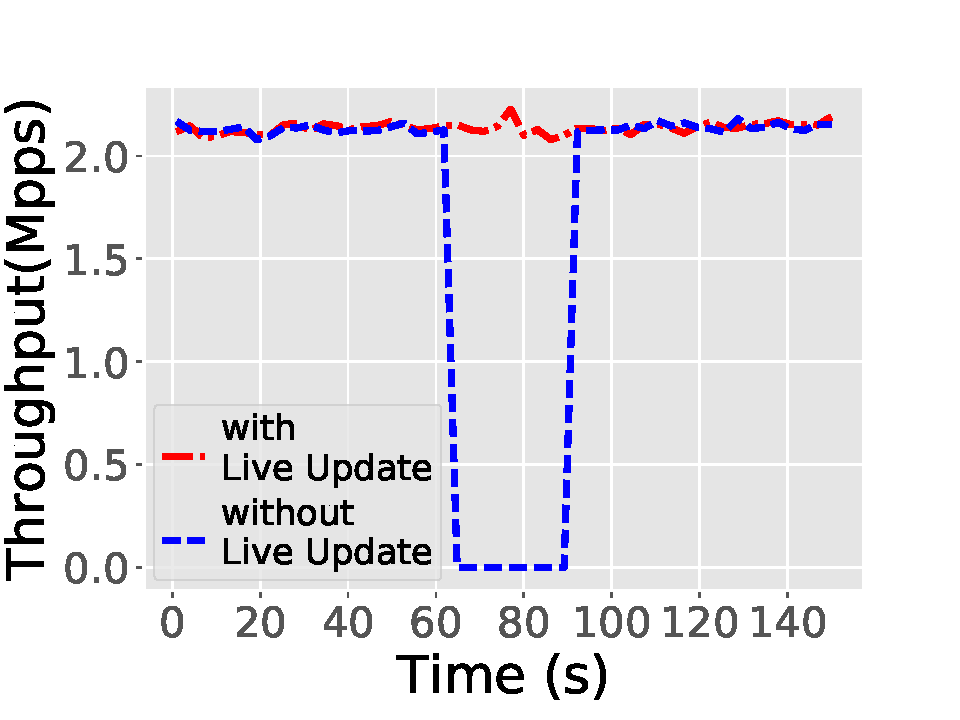
\includegraphics[width=0.7\columnwidth]{figure/Dynamic.pdf}
   %\caption{The packet processing throughput when dynamically update the firewall rule of a runtime configured with firewall NF. }
   \caption{}\label{fig:dynamic-update}
  \end{subfigure}\hfill
  \begin{subfigure}[t]{\linewidth}
 \centering
   \includegraphics[width=0.75\columnwidth]{figure/MPTCP.pdf}
   %\caption{Total number of correctly processed MPTCP flows by three runtimes when MPTCP detection is enabled on runtimes or disabled on runtimes.}
   \vspace{-2mm}
   \caption{}\label{fig:mptcp} \end{subfigure}%\hfill
  %\begin{subfigure}[t]{0.33\linewidth}
% \centering
 %  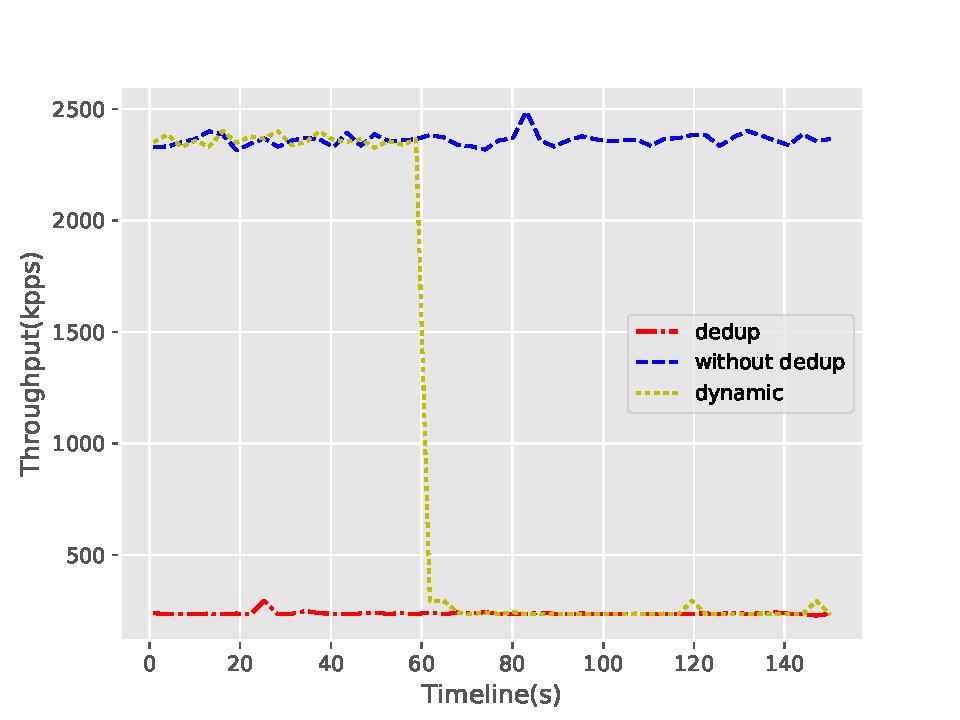
\includegraphics[width=\columnwidth]{figure/Dedup.pdf}
   %\caption{The output throughput of three runtimes when deduplication is disabled, enabled or enabled half way. }
 %  \caption{}\label{fig:deduplication} \end{subfigure}
 \vspace{-2mm}
 \caption{New applications enabled with distributed flow migration capability of \nfactor.}
\label{fig:rep-perf}
\end{figure}

%The final application is similar with MPTCP application, which reduces the output bandwidth for deduplication.

%\vspace{1mm}
%\noindent\textbf{Flow Deduplication.} Flow deduplication, as an important functionality of WAN optimizers \cite{anand2010cheap}, is useful for reducing bandwidth consumption due to transfer redundant data across different flows. \nfactor~can efficiently support flow deduplication: when a runtime receives a flow, it checks for duplicated content contained in the flow packet by performing a consistent hash over the entire packet content. \chuan{how does it check duplicated content among different flows received on different runtimes? otherwise, duplicate with whom?}.
%If duplication identified, the flow actor initiates a migration to move the flow to a specific runtime, as indicated by the hash value of the packet content. In this way, duplicated flows can be processed on the same runtime, eliminating redundant processing and bandwidth consumption. When the duplicated flows arrive on the same runtime, before the packets are sent out from the runtime, we use the liason actor to intercept duplicated packet, and only generate an output data packet for every 10 duplicated packet it receives. The output data packet is packed with useful information (\ie packet header of dupliated packet plus an identifier for identifying the duplicated content), so that the receiver on the other end could reconstruct all the original duplicated packets.
%Figure~\ref{fig:deduplication} illustrates deduplication performance. We can see that deduplication decreases the number of output packets by around 90\% through effective deduplication.
 %actors send the output packet out, the runtime intercepts duplicated content,  \chuan{why processing duplicated flows on the same runtime can reduce output bandwidth? Are they processed by the same flow actor? what if the flows are partially duplicated but not entirely?}. This is hard to be achieved in existing NFV systems because xxx \chuan{give the reason}.
